% Options for packages loaded elsewhere
\PassOptionsToPackage{unicode}{hyperref}
\PassOptionsToPackage{hyphens}{url}
\PassOptionsToPackage{dvipsnames,svgnames*,x11names*}{xcolor}
%
\documentclass[
  10pt,
]{krantz}
\usepackage{amsmath,amssymb}
\usepackage{lmodern}
\usepackage{ifxetex,ifluatex}
\ifnum 0\ifxetex 1\fi\ifluatex 1\fi=0 % if pdftex
  \usepackage[T1]{fontenc}
  \usepackage[utf8]{inputenc}
  \usepackage{textcomp} % provide euro and other symbols
\else % if luatex or xetex
  \usepackage{unicode-math}
  \defaultfontfeatures{Scale=MatchLowercase}
  \defaultfontfeatures[\rmfamily]{Ligatures=TeX,Scale=1}
  \setmonofont[Scale=0.7]{Source Code Pro}
\fi
% Use upquote if available, for straight quotes in verbatim environments
\IfFileExists{upquote.sty}{\usepackage{upquote}}{}
\IfFileExists{microtype.sty}{% use microtype if available
  \usepackage[]{microtype}
  \UseMicrotypeSet[protrusion]{basicmath} % disable protrusion for tt fonts
}{}
\makeatletter
\@ifundefined{KOMAClassName}{% if non-KOMA class
  \IfFileExists{parskip.sty}{%
    \usepackage{parskip}
  }{% else
    \setlength{\parindent}{0pt}
    \setlength{\parskip}{6pt plus 2pt minus 1pt}}
}{% if KOMA class
  \KOMAoptions{parskip=half}}
\makeatother
\usepackage{xcolor}
\IfFileExists{xurl.sty}{\usepackage{xurl}}{} % add URL line breaks if available
\IfFileExists{bookmark.sty}{\usepackage{bookmark}}{\usepackage{hyperref}}
\hypersetup{
  pdftitle={Elementos de la estadística},
  pdfauthor={Ricardo Michel MALLQUI BAÑOS},
  colorlinks=true,
  linkcolor=Maroon,
  filecolor=Maroon,
  citecolor=Blue,
  urlcolor=Blue,
  pdfcreator={LaTeX via pandoc}}
\urlstyle{same} % disable monospaced font for URLs
\usepackage{color}
\usepackage{fancyvrb}
\newcommand{\VerbBar}{|}
\newcommand{\VERB}{\Verb[commandchars=\\\{\}]}
\DefineVerbatimEnvironment{Highlighting}{Verbatim}{commandchars=\\\{\}}
% Add ',fontsize=\small' for more characters per line
\usepackage{framed}
\definecolor{shadecolor}{RGB}{248,248,248}
\newenvironment{Shaded}{\begin{snugshade}}{\end{snugshade}}
\newcommand{\AlertTok}[1]{\textcolor[rgb]{0.94,0.16,0.16}{#1}}
\newcommand{\AnnotationTok}[1]{\textcolor[rgb]{0.56,0.35,0.01}{\textbf{\textit{#1}}}}
\newcommand{\AttributeTok}[1]{\textcolor[rgb]{0.77,0.63,0.00}{#1}}
\newcommand{\BaseNTok}[1]{\textcolor[rgb]{0.00,0.00,0.81}{#1}}
\newcommand{\BuiltInTok}[1]{#1}
\newcommand{\CharTok}[1]{\textcolor[rgb]{0.31,0.60,0.02}{#1}}
\newcommand{\CommentTok}[1]{\textcolor[rgb]{0.56,0.35,0.01}{\textit{#1}}}
\newcommand{\CommentVarTok}[1]{\textcolor[rgb]{0.56,0.35,0.01}{\textbf{\textit{#1}}}}
\newcommand{\ConstantTok}[1]{\textcolor[rgb]{0.00,0.00,0.00}{#1}}
\newcommand{\ControlFlowTok}[1]{\textcolor[rgb]{0.13,0.29,0.53}{\textbf{#1}}}
\newcommand{\DataTypeTok}[1]{\textcolor[rgb]{0.13,0.29,0.53}{#1}}
\newcommand{\DecValTok}[1]{\textcolor[rgb]{0.00,0.00,0.81}{#1}}
\newcommand{\DocumentationTok}[1]{\textcolor[rgb]{0.56,0.35,0.01}{\textbf{\textit{#1}}}}
\newcommand{\ErrorTok}[1]{\textcolor[rgb]{0.64,0.00,0.00}{\textbf{#1}}}
\newcommand{\ExtensionTok}[1]{#1}
\newcommand{\FloatTok}[1]{\textcolor[rgb]{0.00,0.00,0.81}{#1}}
\newcommand{\FunctionTok}[1]{\textcolor[rgb]{0.00,0.00,0.00}{#1}}
\newcommand{\ImportTok}[1]{#1}
\newcommand{\InformationTok}[1]{\textcolor[rgb]{0.56,0.35,0.01}{\textbf{\textit{#1}}}}
\newcommand{\KeywordTok}[1]{\textcolor[rgb]{0.13,0.29,0.53}{\textbf{#1}}}
\newcommand{\NormalTok}[1]{#1}
\newcommand{\OperatorTok}[1]{\textcolor[rgb]{0.81,0.36,0.00}{\textbf{#1}}}
\newcommand{\OtherTok}[1]{\textcolor[rgb]{0.56,0.35,0.01}{#1}}
\newcommand{\PreprocessorTok}[1]{\textcolor[rgb]{0.56,0.35,0.01}{\textit{#1}}}
\newcommand{\RegionMarkerTok}[1]{#1}
\newcommand{\SpecialCharTok}[1]{\textcolor[rgb]{0.00,0.00,0.00}{#1}}
\newcommand{\SpecialStringTok}[1]{\textcolor[rgb]{0.31,0.60,0.02}{#1}}
\newcommand{\StringTok}[1]{\textcolor[rgb]{0.31,0.60,0.02}{#1}}
\newcommand{\VariableTok}[1]{\textcolor[rgb]{0.00,0.00,0.00}{#1}}
\newcommand{\VerbatimStringTok}[1]{\textcolor[rgb]{0.31,0.60,0.02}{#1}}
\newcommand{\WarningTok}[1]{\textcolor[rgb]{0.56,0.35,0.01}{\textbf{\textit{#1}}}}
\usepackage{longtable,booktabs,array}
\usepackage{calc} % for calculating minipage widths
% Correct order of tables after \paragraph or \subparagraph
\usepackage{etoolbox}
\makeatletter
\patchcmd\longtable{\par}{\if@noskipsec\mbox{}\fi\par}{}{}
\makeatother
% Allow footnotes in longtable head/foot
\IfFileExists{footnotehyper.sty}{\usepackage{footnotehyper}}{\usepackage{footnote}}
\makesavenoteenv{longtable}
\setlength{\emergencystretch}{3em} % prevent overfull lines
\providecommand{\tightlist}{%
  \setlength{\itemsep}{0pt}\setlength{\parskip}{0pt}}
\setcounter{secnumdepth}{5}
\usepackage[spanish,es-lcroman,es-tabla]{babel}
\usepackage{booktabs}
\usepackage{graphicx} 
\usepackage{amsmath}
\usepackage{makeidx}
\usepackage{array}% http://ctan.org/pkg/array
\makeindex

\makeatletter\@addtoreset{chapter}{part}\makeatother%

%\usepackage{showframe}
%\usepackage[a4paper]{geometry}
%\geometry{verbose,tmargin=3cm,bmargin=3cm,lmargin=3.5cm,rmargin=3cm}
\setlength{\tabcolsep}{0.38em}
%\renewcommand{\arraystretch}{1.5}

\usepackage{times}
\renewcommand{\rmdefault}{ptm}
%\usepackage[lite,subscriptcorrection,nofontinfo,zswash]{mtpro2}

\usepackage{graphicx}

% Determine if the image is too wide for the page.
\makeatletter
\def\ScaleIfNeeded{%
  \ifdim\Gin@nat@width>\linewidth
    \linewidth
  \else
    \Gin@nat@width
  \fi
}
\makeatother

% Resize figures that are too wide for the page.
\let\oldincludegraphics\includegraphics
\renewcommand\includegraphics[2][]{%
  \oldincludegraphics[scale=0.85]{#2}
}

\usepackage{amsthm}
\makeatletter
\def\thm@space@setup{%
  \thm@preskip=8pt plus 2pt minus 4pt
  \thm@postskip=\thm@preskip
}
\makeatother



%\flushbottom 

\frontmatter

\ifluatex
  \usepackage{selnolig}  % disable illegal ligatures
\fi
\usepackage[]{natbib}
\bibliographystyle{apalike}

\title{Elementos de la estadística}
\usepackage{etoolbox}
\makeatletter
\providecommand{\subtitle}[1]{% add subtitle to \maketitle
  \apptocmd{\@title}{\par {\large #1 \par}}{}{}
}
\makeatother
\subtitle{estadística descriptiva y probabilidades}
\author{Ricardo Michel MALLQUI BAÑOS}
\date{2021-09-11}

\usepackage{amsthm}
\newtheorem{theorem}{Teorema}[chapter]
\newtheorem{lemma}{Lema}[chapter]
\newtheorem{corollary}{Corolario}[chapter]
\newtheorem{proposition}{Proposición}[chapter]
\newtheorem{conjecture}{Conjectura}[chapter]
\theoremstyle{definition}
\newtheorem{definition}{Definición}[chapter]
\theoremstyle{definition}
\newtheorem{example}{Ejemplo}[chapter]
\theoremstyle{definition}
\newtheorem{exercise}{Ejercicio}[chapter]
\theoremstyle{definition}
\newtheorem{hypothesis}{Hypothesis}[chapter]
\theoremstyle{remark}
\newtheorem*{remark}{Observación}
\newtheorem*{solution}{Solución}
\begin{document}
\maketitle

%\cleardoublepage\newpage\thispagestyle{empty}\null
%\cleardoublepage\newpage\thispagestyle{empty}\null
%\cleardoublepage\newpage
\thispagestyle{empty}
\begin{center}

\includegraphics{U.pdf}
\end{center}

%\setlength{\abovedisplayskip}{-5pt}
%\setlength{\abovedisplayshortskip}{-5pt}

{
\hypersetup{linkcolor=}
\setcounter{tocdepth}{2}
\tableofcontents
}
\listoftables
\listoffigures
\newcommand{\N}{\mathbb{N}}
\newcommand{\R}{\mathbb{R}}
\newcommand{\CC}{\mathbb{C}}
\newcommand{\I}{\mathbb{I}}
\newcommand{\f}{\mathbb{f}}
\newcommand{\X}{\mathbb{X}}
\newcommand{\D}{\mathbb{D}}
\newcommand{\Z}{\mathbb{Z}}
\newcommand{\Q}{\mathbb{Q}}
\newcommand{\norm}[1]{\left\Vert#1\right\Vert}
\newcommand{\abs}[1]{\left\vert#1\right\vert}
\newcommand{\set}[1]{\left\{#1\right\}}
\newcommand{\seq}[1]{\left<#1\right>}
\newcommand{\co}[1]{\left[#1\right]}
\newcommand{\cc}[1]{\left(#1\right)}
\newcommand{\J}{\mathcal{J}}
\newcommand{\K}{\mathcal{K}}
\newcommand{\M}{\mathcal{M}}
\newcommand{\F}{\mathcal{F}}

\hypertarget{resumen}{%
\chapter*{Resumen}\label{resumen}}


La estadística es la ciencia que manipula datos las analiza e interpreta para poder sacar concluciones razonables de ciertos fenomenos naturales. Esta ciencia puede ser dividido en dos: \textbf{estadística descirptiva} y \textbf{estadística inferencial}. En la estadística descriptiva se procesan datos de una manera teórica y utilitaria. Estos métodos consisten en la recolección, organización, resumen, descripcion y presenatacion de la información. Si la poblacion está disponible entonces la estadística descriptiva es suficiente para describir ciertos fenomenos. No obstante generalmente no se dispone de toda la población si no de una muestra de ella, es en este caso que se requieren usar técnicas más sofisticadas para tomar decisiones y generalizaciones acerca de la poblacion, desde una pequeña muestra de información. Es cuando entra en el juego la estadística inferencial.

La base teórica de la estadística son las matemáticas

Este libro se compone de dos partes, la primera parte trata sobre la \textbf{estadística descirptiva} y la segunda \textbf{estadística inferencial}. Cada una de ellas divididas en capítulos.

\mainmatter

\hypertarget{part-estaduxedstica-descriptiva}{%
\part{Estadística descriptiva}\label{part-estaduxedstica-descriptiva}}

\hypertarget{prerrequisitos}{%
\chapter{Prerrequisitos}\label{prerrequisitos}}

WWWWWWWWWWWWWWWWWWWWWWWWWWWWWWWWWWWW

\hypertarget{variables}{%
\chapter{Variables}\label{variables}}

Es una \textbf{característica} de personas cosas u objetos que son propensos a ser medidas o cualificadas

\hypertarget{variables-cualitativas}{%
\section{Variables cualitativas}\label{variables-cualitativas}}

Denotan cualidades de objetos personas o animales tales como características inherentes que \emph{no son medibles por números}, tenemos dos casos de esta variable.

\hypertarget{nominales}{%
\subsection{Nominales}\label{nominales}}

Son caracteristicas que simplemente nominan y están propensos a ser jerarquizados u ordenados tales como: El estado civil (soltero, casado, divorciado, viudo), Religión (católica, evangélico, judío, etc).

\hypertarget{ordinales}{%
\subsection{Ordinales}\label{ordinales}}

Son caracteristicas que que si están propensos a ser jerarquizados tales como: Nivel de instrucción (inicial, primaria, secundaria, superior).

\hypertarget{variables-cuantitativas}{%
\section{Variables cuantitativas}\label{variables-cuantitativas}}

Son aquellas variables que están propensos a ser medidas mediante números ya sean números enteros o reales.

\hypertarget{discretas}{%
\subsection{Discretas}\label{discretas}}

Aquellas que solo son medidos mediante numeros enteros por ejemplo: Número de hijos, número de habitaciones.

\hypertarget{continuas}{%
\subsection{Continuas}\label{continuas}}

Aquellas que solo son medidos mediante numeros reales es decir este incluye a los numeros racionales e irracionales. Estatura, volumen, peso.

\hypertarget{asignaciuxf3n}{%
\section{Asignación}\label{asignaciuxf3n}}

\begin{enumerate}
\def\labelenumi{\arabic{enumi}.}
\item
  Reconosca \textbf{5} variables \textbf{cualitativas} de una persona, admosfera, una pintura

  \begin{itemize}
  \tightlist
  \item
    Persona

    \begin{itemize}
    \tightlist
    \item
      Color (moreno, blanco, trigueo)
    \item
      Religión (catolico, evangelico, pentecostal, etc)
    \item
      wwwwwww
    \item
      wwww
    \item
      wwwwww
    \end{itemize}
  \item
    Admosfera

    \begin{itemize}
    \tightlist
    \item
      www
    \item
      wwwww
    \item
      wwwwwww
    \item
      wwww
    \item
      wwwwww
    \end{itemize}
  \item
    Pintura

    \begin{itemize}
    \tightlist
    \item
      www
    \item
      wwwww
    \item
      wwwwwww
    \item
      wwww
    \item
      wwwwww
    \end{itemize}
  \end{itemize}
\item
  Reconosca \textbf{5} variables \textbf{cuantitativas} de una video, tela, un celular.

  \begin{itemize}
  \tightlist
  \item
    Video

    \begin{itemize}
    \tightlist
    \item
      Duracion (\(x\) segundos)
    \item
      Numero video en youtube a la semana (\(n\) cantidades)
    \item
      wwwwwww
    \item
      wwww
    \item
      wwwwww
    \end{itemize}
  \item
    Tela

    \begin{itemize}
    \tightlist
    \item
      www
    \item
      wwwww
    \item
      wwwwwww
    \item
      wwww
    \item
      wwwwww
    \end{itemize}
  \item
    Celular

    \begin{itemize}
    \tightlist
    \item
      www
    \item
      wwwww
    \item
      wwwwwww
    \item
      wwww
    \item
      wwwwww
    \end{itemize}
  \end{itemize}
\end{enumerate}

\hypertarget{organizaciuxf3n-de-datos-en-tablas-de-frecuencias}{%
\chapter{Organización de datos en tablas de frecuencias}\label{organizaciuxf3n-de-datos-en-tablas-de-frecuencias}}

\hypertarget{distribuciuxf3n-de-frecuencias}{%
\section{Distribución de frecuencias}\label{distribuciuxf3n-de-frecuencias}}

La tabulación es un proceso en el cual los datos son ordenados en grupos llamados \emph{clases} para un análisis más eficaz de estos, los datos podrían estar clasificados mediante una variable cualitativa o cuantitativa en el caso de las variables cualitativas \(Y_i\), se considera la siguiente Tabla \ref{tab:ww}

\begin{longtable}[]{@{}cccccccccc@{}}
\caption{\label{tab:ww} Caption}\tabularnewline
\toprule
\(Y_i\) & \(f_i\) & \(F_i\) & \(F_i^*\) & \(h_i\) & \(H_i\) & \(H_i^*\) & \(h_i\%\) & \(H_i\%\) & \(H_i^*\%\) \\
\midrule
\endfirsthead
\toprule
\(Y_i\) & \(f_i\) & \(F_i\) & \(F_i^*\) & \(h_i\) & \(H_i\) & \(H_i^*\) & \(h_i\%\) & \(H_i\%\) & \(H_i^*\%\) \\
\midrule
\endhead
\(Y_1\) & \(f_1\) & \(F_1\) & \(F_1^*\) & \(\frac{f_1}{n}\) & \(\frac{F_1}{n}\) & \(\frac{F_1^*}{n}\) & \(h_1\) & \(H_1\) & \(H_1^*\) \\
\(Y_2\) & \(f_2\) & \(F_2\) & \(F_2^*\) & \(\frac{f_2}{n}\) & \(\frac{F_2}{n}\) & \(\frac{F_2^*}{n}\) & \(h_2\) & \(H_2\) & \(H_1^*\) \\
\(Y_3\) & \(f_3\) & \(F_3\) & \(F_3^*\) & \(\frac{f_3}{n}\) & \(\frac{F_3}{n}\) & \(\frac{F_3^*}{n}\) & \(h_3\) & \(H_3\) & \(H_1^*\) \\
\(\vdots\) & \(\vdots\) & \(\vdots\) & \(\vdots\) & \(\vdots\) & \(\vdots\) & \(\vdots\) & \(\vdots\) & \(\vdots\) & \(\vdots\) \\
\(Y_r\) & \(f_r\) & \(F_r\) & \(F_r^*\) & \(\frac{f_r}{n}\) & \(\frac{F_r}{n}\) & \(\frac{F_r^*}{n}\) & \(h_r\) & \(H_r\) & \(H_1^*\) \\
\bottomrule
\end{longtable}

En el caso de variables cuantitativas ademas si los datos son muy variados, que para se clasificados adecuadamente, necesitan generarse particiones de longitudes semejantes entonces se utiliza el siguiente proceso; el \textbf{número de las particiones} \(r\) se consideran de acuerdo a \textbf{tres criterios}

\begin{enumerate}
\def\labelenumi{\arabic{enumi}.}
\item
  Criterio del investigador \(r\) no puede ser más de 20 ni menos de 5
\item
  \(r=\sqrt{n}\) donde \(n\) es el número de datos
\item
  La regla de Starges que consiste en considerar la fórmula \(r=3.322\cdot\log_{10} n\)
  Una vez establecido el número de particiones se procede a generar los límites laterales de cada una de las particiones, sea \(L\) la longitud de todo el conjunto es decir \(L=x_{\text{max}}-x_{\text{min}}\) entonces la longitud de las particiones o amplitud interválica se obtiene con \(l=\frac{L}{r}\)
\end{enumerate}

\begin{longtable}[t]{ccccccccccc}
\caption{\label{tab:cuantitativaw}Datos cuantitativos (intervalos)}\\
\toprule
Clase & $Y_i$ & $f_i$ & $F_i$ & $F_i^*$ & $h_i$ & $H_i$ & $H_i^*$ & $h_i\%$ & $H_i\%$ & $H_i^*\%$\\
\midrule
$[y_1-y_2)$ & $Y_1$ & $f_i$ & $F_i$ & $F_i^*$ & $\frac{f_1}{n}$ & $\frac{f_1}{n}$ & $\frac{F_1^*}{n}$ & $h_1\%$ & $H_1\%$ & $H_1^*\%$\\
$[y_2-y_3)$ & $Y_2$ & $f_i$ & $F_i$ & $F_i^*$ & $\frac{f_2}{n}$ & $\frac{f_1}{n}$ & $\frac{F_1^*}{n}$ & $h_2\%$ & $H_2\%$ & $H_2^*\%$\\
$\ldots$ & $\ldots$ & $\ldots$ & $\ldots$ & $\ldots$ & $\ldots$ & $\ldots$ & $\ldots$ & $\ldots$ & $\ldots$ & $\ldots$\\
$[y_{r-1}-y_r)$ & $Y_r$ & $f_r$ & $F_r$ & $F_r^*$ & $\frac{f_r}{n}$ & $\frac{f_1}{n}$ & $\frac{F_r^*}{n}$ & $h_r\%$ & $H_r\%$ & $H_r^*\%$\\
\bottomrule
\end{longtable}

Tenga en cuenta que \(n\) es el número de datos, es decir \(n=f_1+f_2+\ldots+f_r=\sum_{i=1}^r\) donde \(f_i\) es número de datos en la partición \(X_i\), una de las \(r\) particiones del conjunto total de datos.

\begin{enumerate}
\def\labelenumi{\arabic{enumi}.}
\item
  Las \textbf{frecuencias absolutas}\index{frecuencias absolutas} \(f_i\) indican el número de datos con la característica \(X_i\).
\item
  Las \textbf{frecuencias absolutas acumuladas menor que}\index{frecuencias absolutas acumuladas menor que} \(F_i\) obedecen a la fórmula
  \[F_m=f_1+f_2+\ldots+f_m=\sum_{i=1}^mf_i\]
\item
  Las \textbf{frecuencias absolutas acumuladas mayor que} \(F_i^*\) obedecen a la fórmula
  \[
  \begin{aligned}
  F_m^*&=f_m+f_{m+1}+\ldots+f_r\\
  &=\sum_{i=m}^rf_i\\
  &=n-\sum_{i=1}^{m-1}f_i\\
  &=n-\left(f_1+f_{2}+\ldots+f_{m-1}\right)
  \end{aligned} 
  \]
\item
  Las \textbf{frecuencias absolutas relativas}\index{frecuencias absolutas relativas} obedecen a la fórmula
  \[h_m=\frac{f_m}{n}\]
\item
  Las \textbf{frecuencias absolutas relativas menor que}\index{frecuencias absolutas relativas  menor que} obedecen a la fórmula
  \[H_m=\frac{f_m}{n}\]
\item
  Las \textbf{frecuencias absolutas relativas mayor que} obedecen a la fórmula
  \[H_m^*=\frac{F_m}{n}\]
\item
  Las \textbf{frecuencias absolutas relativas porcentuales} obedecen a la fórmula
  \(h_i\%=100\cdot h_i\)
\item
  Las \textbf{frecuencias absolutas relativas menor que porcentuales} obedecen a la fórmula
  \(H_i\%=100\cdot H_i\)
\item
  Las \textbf{frecuencias absolutas relativas mayor que porcentuales} obedecen a la fórmula
  \(H_i^*\%=100\cdot H_i^*\)
\end{enumerate}

\hypertarget{ejemplo-sin-intervalos}{%
\section{Ejemplo sin intervalos}\label{ejemplo-sin-intervalos}}

\begin{exercise}
\protect\hypertarget{exr:unnamed-chunk-1}{}{\label{exr:unnamed-chunk-1} }Sean Los 16 tipos de personalidad en un grupo social encuestado.

\begin{enumerate}
\def\labelenumi{\arabic{enumi}.}
\item
  ESTJ (Extraverted Sensing Thinking Judging)
  Personas a las que les gusta tener el control sobre lo que ocurre a su alrededor, siempre buscan la manera de que todo funcione como debe y, si es necesario, la implementan ellos mismos.
\item
  ESTP ((Extraverted Sensing Thinking Perceiving)
  Las personas que pertenecen a esta categoría son espontáneas, alegres y activas, pero al igual que lo que ocurre con los ESTJ, tienden a ejercer dominio sobre los demás, en este caso a través de su capacidad de observación y su carisma.
\item
  ESFJ (Extraverted Sensing Feeling Judging)
  Se trata de personas muy volcadas en la atención de las necesidad de los demás, especialmente si forman parte de su círculo cercano: familia y amistades. Por eso siempre que pueden prestan su ayuda y procuran que sus círculos sociales cercanos permanezcan siempre estables y con buena salud. Por eso tienden a evitar que aparezcan conflictos fuertes y se muestran diplomáticas cuando hay choques de intereses.
\item
  ESFP (Extraverted Sensing Feeling Perceiving)
  Se trata de personas alegres y espontáneas que disfrutan entreteniéndose y entreteniendo a los demás. La diversión es uno de los pilares más importantes de sus vidas, y son de trato cercano y temperamento cálido. Aman la novedad y hablar acerca de experiencias personales.
\item
  ISTJ (Introverted Sensing Thinking Perceiving)
  Un tipo de personalidad definido por su fuerte sentido de la moralidad y del deber. Les gusta planear e implementar sistemas de reglas que permitan que equipos y organizaciones funcionen con una clara lógica y orden. Dan un gran valor a las normas y a la necesidad de que la realidad se corresponda con cómo deberían ser las cosas. Aunque son personas introvertidas, no rehuyen la interacción con los demás.
\item
  ISTP (Introverted Sensing Thinking Perceiving)
  Se trata de personas reservadas, orientadas a la acción y a las soluciones prácticas ante problemas del día a día. También son definidas por su tendencia hacia el pensamiento lógico y su espontaneidad y autonomía. Les gusta explorar entornos y descubrir modos en los que se puede interactuar con ellos.
\item
  ISFJ (Introverted Sensing Feeling Judging)
  Son personas definidas principalmente por sus ganas de proteger y ayudar a los demás y, en definitiva, de resultar confiables para los otros.Se esfuerzan por hacer todo lo que se espera de ellas, pero no tienen grandes aspiraciones ni se muestran muy ambiciosas. Tienden a pensar que es malo pedir compensaciones o aumentos a cambio de los sacrificios que realizan a la hora de trabajar, ya que este debería ser una meta en sí.
\item
  ISFP (Introverted Sensing Feeling Perceiving)
  Personas que viven totalmente en el aquí y el ahora, en constante búsqueda de la novedad y de las situaciones sensorialmente estimulantes. Son reservadas, pero también alegres, espontáneas y cálidas con sus amistades.Tienen un especial talento en el mundo de las artes.
\item
  ENTJ (Extraverted Intuitive Thinking Judging)
  Este es uno de los 16 tipos de personalidad más relacionados con el liderazgo y la asertividad. Las personas descritas por esta categoría son comunicativas, de pensamiento ágil y analítico y predispuestas a encabezar equipos y organizaciones. Se adaptan bien al cambio y hacen que sus estrategias también se amolden cada vez que el entorno varía. Además, casi siempre saben cómo explicar sus proyectos o historias de manera que resulten de interés para el resto, lo cual los convierte en comerciales muy aptos.
\item
  ENTP (Extraverted Intuitive Thinking Perceiving)
  Personas especialmente movidas por la curiosidad y por los retos que para ser resueltos requieren afrontar preguntas intelectualmente estimulantes. Su agilidad mental y su facilidad para detectar inconsistencias lógicas hace de ellas personas predispuestas a interesarse por la ciencia o la filosofía. Además, su tendencia a mostrarse competitivas las vuelve personas muy activas durante el día, siempre intentando llegar a soluciones innovadoras a problemas complejos.
\item
  ENFJ (Extraverted Intuitive Feeling Judging)
  Personas que aprenden constantemente acerca de todos los ámbitos del conocimiento (o una buena parte de ellas) y ayudan a aprender a las demás, guiándolas en su propia evolución. Les gusta ofrecer tutela y consejo, y son muy buenas influyendo en la conducta de los demás. Se centran en sus valores e ideales y hacen lo posible por mejorar el bienestar del mayor número de personas a través de sus ideas y sus acciones.
\item
  ENFP (Extraverted Intuitive Feeling Perceiving)
  Uno de los 16 tipos de personalidad con mayor propensión al pensamiento creativo, las artes y a la sociabilidad. Son alegres, disfrutan de la interacción con otras personas, y actúan teniendo en mente su posición como parte de un ``todo'' formado por la humanidad, y no se muestran individualistas. De hecho, suelen involucrarse en tareas colectivas para ayudar a los demás, pensando en el impacto social de sus acciones. Sin embargo, también se distraen fácilmente y es frecuente que posterguen tareas que consideran aburridas o demasiado simples y rutinarias.
\item
  INTJ (Introverted Intuitive Thinking Judging)
  Un tipo de personalidad orientado hacia la resolución de problemas específicos a partir del razonamiento analítico. Las descritas por esta categoría son personas muy centradas en sus propias ideas y teorías acerca del funcionamiento del mundo, lo cual significa que analizan su entorno centrándose en sus ideas sobre cómo opera este. Son conocedoras de sus propias capacidades y confían en su propio criterio, aunque este vaya en contra de algunos superiores.
\end{enumerate}

Es muy frecuente que lleguen a ser expertas en un ámbito de conocimiento muy específico, ya que les gusta tener el suficiente conocimiento sobre algo como para poder tener en cuenta todos los factores que entran en juego en su funcionamiento y, a partir de ahí, saber lo que se puede hacer o lo que pasará en el futuro.

\begin{enumerate}
\def\labelenumi{\arabic{enumi}.}
\setcounter{enumi}{13}
\item
  INTP (Introverted Intuitive Thinking Perceiving)
  Uno de los 16 tipos de personalidad más definido por la propensión a la reflexión. A estas personas les gustan las teorías con capacidad para explicar todo lo que puede ocurrir en un sistema, y su tendencia hacia el perfeccionismo hace que corrijan a los demás en múltiples ocasiones. Valoran más la exactitud en términos teóricos que el pragmatismo y la resolución de problemas concretos.
\item
  INFJ (Introverted Intuitive Feeling Judging)
  Personas muy sensibles, reservadas y movidas por unos ideales muy definidos y que, además, sienten la necesidad de hacer que los demás también se beneficien de estos ideales. Esto hace que sean propensas tanto a la reflexión como a la acción, lo cual puede llegar a suponer tanto trabajo que se sobrecargan por tener demasiadas responsabilidades. Muestran una gran capacidad para interpretar exitosamente los estados mentales de los demás y tratan de utilizar esta información para ayudarlas antes de que la otra persona se lo pida.
\item
  INFP (Introverted Intuitive Feeling Perceiving)
  Menos moralistas que los INFJ, los INFP también se preocupan mucho por ayudar a los demás desde su posición de personas reservadas. Muestran una sensibilidad estética y artística que las vuelve creativas.
\end{enumerate}
\end{exercise}

\begin{solution}
\iffalse{} {Solución. } \fi{}
Se tiene 16 características con los siguientes datos

\begin{longtable}[]{@{}cc@{}}
\toprule
Personalidad & Cantidad \\
\midrule
\endhead
ESTJ & 1 \\
ESTJ & 2 \\
ESTP & 3 \\
ESFJ & 4 \\
ESFP & 5 \\
ISTJ & 6 \\
ISTP & 7 \\
ISFJ & 8 \\
ISFP & 9 \\
ENTJ & 10 \\
ENTP & 6 \\
ENFJ & 5 \\
ENFP & 3 \\
INTJ & 2 \\
INTP & 1 \\
INFJ & 1 \\
INFP & 1 \\
\bottomrule
\end{longtable}
\end{solution}

\begin{longtable}[t]{cccccccccc}
\caption{\label{tab:cualitativa}Datos cualitativos}\\
\toprule
$Y_i$ & $f_i$ & $F_i$ & $F_i^*$ & $h_i$ & $H_i$ & $H_i^*$ & $h_i\%$ & $H_i\%$ & $H_i^*\%$\\
\midrule
ESTJ & 1 & 1 & 75 & 0.01 & 0.01 & 1.00 & 1.33 & 1.33 & 100.00\\
ESTJ & 2 & 3 & 150 & 0.03 & 0.04 & 2.00 & 2.67 & 4.00 & 200.00\\
ESTP & 3 & 6 & 150 & 0.04 & 0.08 & 2.00 & 4.00 & 8.00 & 200.00\\
ESFJ & 4 & 10 & 150 & 0.05 & 0.13 & 2.00 & 5.33 & 13.33 & 200.00\\
ESFP & 6 & 16 & 150 & 0.08 & 0.21 & 2.00 & 8.00 & 21.33 & 200.00\\
ISTJ & 6 & 22 & 155 & 0.08 & 0.29 & 2.07 & 8.00 & 29.33 & 206.67\\
ISTP & 7 & 29 & 157 & 0.09 & 0.39 & 2.09 & 9.33 & 38.67 & 209.33\\
ISFJ & 8 & 37 & 158 & 0.11 & 0.49 & 2.11 & 10.67 & 49.33 & 210.67\\
ISFP & 9 & 46 & 166 & 0.12 & 0.61 & 2.21 & 12.00 & 61.33 & 221.33\\
ENTJ & 10 & 56 & 166 & 0.13 & 0.75 & 2.21 & 13.33 & 74.67 & 221.33\\
ENTP & 6 & 62 & 166 & 0.08 & 0.83 & 2.21 & 8.00 & 82.67 & 221.33\\
ENFJ & 5 & 67 & 166 & 0.07 & 0.89 & 2.21 & 6.67 & 89.33 & 221.33\\
ENFP & 3 & 70 & 166 & 0.04 & 0.93 & 2.21 & 4.00 & 93.33 & 221.33\\
INTJ & 2 & 72 & 167 & 0.03 & 0.96 & 2.23 & 2.67 & 96.00 & 222.67\\
INTP & 1 & 73 & 169 & 0.01 & 0.97 & 2.25 & 1.33 & 97.33 & 225.33\\
INFJ & 1 & 74 & 172 & 0.01 & 0.99 & 2.29 & 1.33 & 98.67 & 229.33\\
INFP & 1 & 75 & 176 & 0.01 & 1.00 & 2.35 & 1.33 & 100.00 & 234.67\\
TOTAL & 75 &  &  &  &  &  & 100.00 &  & \\
\bottomrule
\end{longtable}

\hypertarget{example-intervalos}{%
\section{Example intervalos}\label{example-intervalos}}

\begin{solution}
\iffalse{} {Solución. } \fi{}
Edades de cierta comunidad

25
35 38
45 47 48
51 52 53 55
60 62 63 66 67
70 71 72 75 77 78
81 88 89
90 99

\begin{longtable}[]{@{}cc@{}}
\toprule
Clase & \(f_i\) \\
\midrule
\endhead
\([20-30>\) & 1 \\
\([30-40>\) & 2 \\
\([40-50>\) & 3 \\
\([50-60>\) & 4 \\
\([60-70>\) & 5 \\
\([70-80>\) & 6 \\
\([80-90>\) & 3 \\
\([90-100]\) & 2 \\
\bottomrule
\end{longtable}
\end{solution}

Tabulando

\begin{longtable}[t]{cccccccccc}
\caption{\label{tab:cuantitativa}Datos cuantitativos (intervalos)}\\
\toprule
Clase & $f_i$ & $F_i$ & $F_i^*$ & $h_i$ & $H_i$ & $H_i^*$ & $h_i\%$ & $H_i\%$ & $H_i^*\%$\\
\midrule
$[20-30)$ & 1 & 1 & 26 & 0.02 & 0.01 & 0.35 & 2.38 & 1.33 & 34.67\\
$[30-40)$ & 2 & 3 & 68 & 0.05 & 0.04 & 0.91 & 4.76 & 4.00 & 90.67\\
$[40-50)$ & 3 & 6 & 68 & 0.07 & 0.08 & 0.91 & 7.14 & 8.00 & 90.67\\
$[50-60)$ & 4 & 10 & 68 & 0.10 & 0.13 & 0.91 & 9.52 & 13.33 & 90.67\\
$[60-70)$ & 5 & 15 & 68 & 0.12 & 0.20 & 0.91 & 11.90 & 20.00 & 90.67\\
$[70-80)$ & 6 & 21 & 84 & 0.14 & 0.28 & 1.12 & 14.29 & 28.00 & 112.00\\
$[80-90)$ & 3 & 24 & 84 & 0.07 & 0.32 & 1.12 & 7.14 & 32.00 & 112.00\\
$[90-100]$ & 2 & 26 & 84 & 0.05 & 0.35 & 1.12 & 4.76 & 34.67 & 112.00\\
TOTAL & 42 &  &  &  &  &  & 61.90 &  & \\
\bottomrule
\end{longtable}

\hypertarget{gruxe1ficos-estaduxedsticos}{%
\chapter{Gráficos estadísticos}\label{gruxe1ficos-estaduxedsticos}}

\hypertarget{histograma-de-frecuencias}{%
\section{Histograma de frecuencias}\label{histograma-de-frecuencias}}

\hypertarget{circulares}{%
\section{Circulares}\label{circulares}}

\hypertarget{histograma-de-frecuencias-1}{%
\section{Histograma de frecuencias}\label{histograma-de-frecuencias-1}}

\hypertarget{medidas-de-tendencia-central}{%
\chapter{Medidas de tendencia central}\label{medidas-de-tendencia-central}}

Son aquellas medidas que buscan un dato representivo central de un conjunto de datos tales como la media, la moda y la mediana.

\hypertarget{la-media-overlinex}{%
\section{\texorpdfstring{La media (\(\overline{x}\))}{La media (\textbackslash overline\{x\})}}\label{la-media-overlinex}}

A veces llamada \emph{promedio aritmético}, es la medida de tendencia central que pondera los datos.

\hypertarget{media-de-datos-no-agrupados}{%
\subsection{Media de datos no agrupados}\label{media-de-datos-no-agrupados}}

Los datos no están agrupados cuando no están ordenados sobre una tabla de distribución de frecuencias. Sean los \(n\) datos \(x_1, x_2, \ldots, x_n\) entonces la media o promedio aritmético se define como
\[ \label{eq:w1} 
\overline{x}=\frac{x_1+x_2+\cdots+x_n}{n}=\frac{1}{n}\sum_{i=1}^nx_i 
\]

\hypertarget{media-de-datos-agrupados}{%
\subsection{Media de datos agrupados}\label{media-de-datos-agrupados}}

Considérese la siguiente tabla de distribucion de frecuencias entonces el promedio es \[\overline{x}=\frac{y_1f_1+y_2f_2+\cdots+y_nf_n}{n}=\frac{1}{n}\sum_{i=1}^ny_if_i\]

\begin{longtable}[]{@{}cccccc@{}}
\caption{\label{tab:www} Captionww}\tabularnewline
\toprule
Clase & \(Y_i\) & \(f_i\) & \(F_i\) & \(\ldots\) & \(H_i^*\%\) \\
\midrule
\endfirsthead
\toprule
Clase & \(Y_i\) & \(f_i\) & \(F_i\) & \(\ldots\) & \(H_i^*\%\) \\
\midrule
\endhead
\([y_1,y_2)\) & \(y_1\) & \(f_1\) & \(\ldots\) & \(\ldots\) & \(H_1^*\%\) \\
\([y_2,y_3)\) & \(y_2\) & \(f_2\) & \(\ldots\) & \(\ldots\) & \(H_1^*\%\) \\
\([y_3,y_4)\) & \(y_3\) & \(f_3\) & \(\ldots\) & \(\ldots\) & \(H_1^*\%\) \\
\(\vdots\) & \(\vdots\) & \(\vdots\) & \(\ldots\) & \(\ldots\) & \(\vdots\) \\
\([y_{r-1},y_r]\) & \(y_r\) & \(f_r\) & \(\ldots\) & \(\ldots\) & \(H_1^*\%\) \\
\bottomrule
\end{longtable}

\begin{exercise}
\protect\hypertarget{exr:unnamed-chunk-4}{}{\label{exr:unnamed-chunk-4} }Si el promedio de \(n\) datos es \(\overline{x}\) entonces el promedio del conjunto inicial más un dato adicional \(x_{n+1}\) es \[\overline{x}'=\frac{n\overline{x}+x_{n+1}}{n+1}\] en general si se adicionan \(r\) datos \(y_1, y_2, \ldots y_r\) entonces el nuevo promedio será \[\overline{x}'=\frac{n\overline{x}+y_{1}+y_2+\ldots+y_r}{n+r}\]
\end{exercise}

\begin{solution}
\iffalse{} {Solución. } \fi{}En efecto sea el promedio
\begin{align*}
\overline{x}'&=\frac{x_1+x_2+\cdots+x_{n+1}}{n+1}\\
&=\frac{n\frac{x_1+x_2+\cdots x_n}{n}+x_{n+1}}{n+1}\\
&=\frac{n\overline{x}+x_{n+1}}{n+1}
\end{align*}
\end{solution}

\hypertarget{la-moda-mo}{%
\section{La moda (Mo)}\label{la-moda-mo}}

El dato que mas se prepite

\hypertarget{moda-de-datos-no-tabulados}{%
\subsection{Moda de datos no tabulados}\label{moda-de-datos-no-tabulados}}

En este caso es dato que más repite en un conjunto de datos dados.

La moda es el dato que más se repite por ejemplo sea el conjunto de datos \(x_1\), \(x_2\), \(x_2\), \(x_2\), \(x_3\) entonces la moda es \(\text{Mo}=x_2\)

\hypertarget{moda-de-datos-tabulados}{%
\subsection{Moda de datos tabulados}\label{moda-de-datos-tabulados}}

La moda es el dato que más se repite por ejemplo sea el conjunto de datos tabulados entonces la moda es \[\text{Mo}=Li+\frac{Li-Ls}{Li+Ls}r\]

\begin{longtable}[]{@{}cccccc@{}}
\caption{\label{tab:wwwww} wwwww}\tabularnewline
\toprule
Clase & \(Y_i\) & \(f_i\) & \(F_i\) & \(\ldots\) & \(H_i^*\%\) \\
\midrule
\endfirsthead
\toprule
Clase & \(Y_i\) & \(f_i\) & \(F_i\) & \(\ldots\) & \(H_i^*\%\) \\
\midrule
\endhead
\([y_1,y_2)\) & \(y_1\) & \(f_1\) & \(\ldots\) & \(\ldots\) & \(H_1^*\%\) \\
\([y_2,y_3)\) & \(y_2\) & \(f_2\) & \(\ldots\) & \(\ldots\) & \(H_1^*\%\) \\
\([y_3,y_4)\) & \(y_3\) & \(f_3\) & \(\ldots\) & \(\ldots\) & \(H_1^*\%\) \\
\(\vdots\) & \(\vdots\) & \(\vdots\) & \(\ldots\) & \(\ldots\) & \(\vdots\) \\
\([y_{r-1},y_r]\) & \(y_r\) & \(f_r\) & \(\ldots\) & \(\ldots\) & \(H_1^*\%\) \\
\bottomrule
\end{longtable}

\hypertarget{la-mediana-me}{%
\section{La mediana (Me)}\label{la-mediana-me}}

\hypertarget{mediana-de-datos-no-tabulados}{%
\subsection{Mediana de datos no tabulados}\label{mediana-de-datos-no-tabulados}}

Obtener la mediana consiste en ordenar los datos de menor a mayor y considerar dos casos: El primero si el número de datos es impar entonces el dato \(x_{\frac{n+1}{2}}\) del conjunto ordenado será la mediana es decir \[\text{Me}=x_{\frac{n+1}{2}}\] de otro lado si el número de datos es par entonces la mediana es la semisuma de los dos datos intermedios es decir \[\text{Me}=\frac{x_{\frac{n}{2}}+x_{\frac{n}{2}+1}}{2}\]

\begin{exercise}
\protect\hypertarget{exr:unnamed-chunk-6}{}{\label{exr:unnamed-chunk-6} }Sean los conjuntos de datos 5, 6, 8, 2, 1, 5, 6, 7, 10, 0, 14 y 20, 25, 6, 5, 19, 5 obtener la mediana de estos conjuntos de datos.
\end{exercise}

\begin{solution}
\iffalse{} {Solución. } \fi{}Al ordenarlos se obtiene el siguiente arreglo 0, 1, 2, 5, 5, 6, 6, 7, 8, 10, 14 y considerando que \(x_1=0\), \(x_2=1\), \(\ldots\), \(x_{11}=14\) en este caso el número de datos es impar entonces el dato \(x_{\frac{11+1}{2}}=x_{6}=6\) el la mediana. De otro lado el segundo conjunto de datos al ser ordenados 5, 5, 6, 19, 20, 25 ademas considerando que \(x_1=5\), \(x_2=5\), \(\ldots\), \(x_6=25\) conducen a obtener la mediana \(\text{Me}=\frac{x_{\frac{6}{2}}+x_{\frac{6}{2}+1}}{2}=\frac{6+19}{2}=12.5\).
\end{solution}

\hypertarget{mediana-de-datos-tabulados}{%
\subsection{Mediana de datos tabulados}\label{mediana-de-datos-tabulados}}

\begin{longtable}[]{@{}cccccc@{}}
\caption{\label{tab:mediana} Mediana}\tabularnewline
\toprule
Clase & \(Y_i\) & \(f_i\) & \(F_i\) & \(\ldots\) & \(H_i^*\%\) \\
\midrule
\endfirsthead
\toprule
Clase & \(Y_i\) & \(f_i\) & \(F_i\) & \(\ldots\) & \(H_i^*\%\) \\
\midrule
\endhead
\([y_1,y_2)\) & \(y_1\) & \(f_1\) & \(\ldots\) & \(\ldots\) & \(H_1^*\%\) \\
\([y_2,y_3)\) & \(y_2\) & \(f_2\) & \(\ldots\) & \(\ldots\) & \(H_1^*\%\) \\
\([y_3,y_4)\) & \(y_3\) & \(f_3\) & \(\ldots\) & \(\ldots\) & \(H_1^*\%\) \\
\(\vdots\) & \(\vdots\) & \(\vdots\) & \(\ldots\) & \(\ldots\) & \(\vdots\) \\
\([y_{r-1},y_r]\) & \(y_r\) & \(f_r\) & \(\ldots\) & \(\ldots\) & \(H_1^*\%\) \\
\bottomrule
\end{longtable}

Los pasos son:

\begin{enumerate}
\def\labelenumi{\arabic{enumi}.}
\tightlist
\item
  Se halla \(\frac{n}{2}\) luego
\item
  \(x_n\)
\end{enumerate}

\hypertarget{medidas-de-dispersiuxf3n}{%
\chapter{Medidas de dispersión}\label{medidas-de-dispersiuxf3n}}

\hypertarget{varianza}{%
\section{Varianza}\label{varianza}}

\hypertarget{medidas-de-asimetruxeda}{%
\chapter{Medidas de asimetría}\label{medidas-de-asimetruxeda}}

\hypertarget{part-probabilidades}{%
\part{Probabilidades}\label{part-probabilidades}}

\hypertarget{experimento-aleatorio}{%
\chapter{Experimento aleatorio}\label{experimento-aleatorio}}

\begin{definition}[Experimento aleatorio]
\protect\hypertarget{def:unnamed-chunk-8}{}{\label{def:unnamed-chunk-8} \iffalse (Experimento aleatorio) \fi{} }En experiento aleatorio es un fenomeno que genera un evento
\end{definition}

\hypertarget{uxe1lgebra-de-eventos}{%
\chapter{Álgebra de eventos}\label{uxe1lgebra-de-eventos}}

Sean \(A\), \(B\) y \(C\) eventos entonces
1. e
2. wwwwwwwwwwwwwwwwwwwwwwwwwwwwww

\[ \int_{1}^{2}=\sum_{2}^{2}x_1 \]

\hypertarget{tuxe9cnicas-de-conteo}{%
\chapter{Técnicas de conteo}\label{tuxe9cnicas-de-conteo}}

\(P_n^m\)
\(C_n^m\)

\[\binom{m}{n}=\frac{m}{n!(n-m)}\]

\hypertarget{definiciuxf3n-de-probabilidad}{%
\chapter{Definición de probabilidad}\label{definiciuxf3n-de-probabilidad}}

\hypertarget{probabilidad-condicional}{%
\chapter{Probabilidad condicional}\label{probabilidad-condicional}}

\[P(A|B)= \frac{P(B\cap A)}{P(B)}\]

\hypertarget{teorema-de-bayes}{%
\chapter{Teorema de Bayes}\label{teorema-de-bayes}}

\begin{theorem}[Teorema de Bayes]
\protect\hypertarget{thm:unnamed-chunk-9}{}{\label{thm:unnamed-chunk-9} \iffalse (Teorema de Bayes) \fi{} }Sea \(\{A_{1},A_{2},...,A_{i},...,A_{n}\}\) un conjunto de sucesos mutuamente excluyentes y exhaustivos, y tales que la probabilidad de cada uno de ellos es distinta de cero (0). Sea \(B\) un suceso cualquiera del que se conocen las probabilidades condicionales \(P(B|A_i )\). Entonces, la probabilidad \(P(A_i|B)\) viene dada por la expresión:
\[P(A_i|B)=\frac{P(B|A_i)P(A_i)}{P(B)}\]
donde:

\begin{enumerate}
\def\labelenumi{\arabic{enumi}.}
\tightlist
\item
  \(P(A_i)\) son las probabilidades a priori,
\item
  \(P(B|A_i)\) es la probabilidad de B en la hipótesis \(A_i\),
\item
  \(P(A_i|B)\) son las probabilidades a posteriori.
\end{enumerate}
\end{theorem}

\hypertarget{eventos-independientes-y-secuencias-de-experimentos}{%
\chapter{Eventos independientes y secuencias de experimentos}\label{eventos-independientes-y-secuencias-de-experimentos}}

\hypertarget{probabilidad-en-espacio}{%
\chapter{Probabilidad en espacio}\label{probabilidad-en-espacio}}

\hypertarget{part-inferencia-estaduxedstica}{%
\part{Inferencia estadística}\label{part-inferencia-estaduxedstica}}

\hypertarget{variables-aleatorias}{%
\chapter{Variables aleatorias}\label{variables-aleatorias}}

\begin{definition}[Variable aleatoria]
\protect\hypertarget{def:unnamed-chunk-10}{}{\label{def:unnamed-chunk-10} \iffalse (Variable aleatoria) \fi{} }Sea \(\Omega\) un espacio muestral asociado a una experimento aleatorio \(\epsilon\) y \(\omega\in\Omega\), entonces se genera la función \textbf{variable aleatoria}
\begin{align*}
  X:\Omega&\longrightarrow \mathbb{R}\\
  \omega&\longmapsto X(\omega)
\end{align*}
\end{definition}
\(R_{X}=\{x\in \mathbb {R} /\ \exists \,\omega \in \Omega :X(\omega )=x\}\)
es decir a cada elemento de \(\Omega\) se le asocia un número real \(\mathbb{R}\), además la probabilidad de \(x\in \mathbb{R}\) es \(P[x]= \sum^{n}_{i=1}P\left[\omega_i\right]\) donde \(\omega_i\in X^{-1}(x)\). La definición indica por otro lado que un espacio muestral \(\Omega\) puede genera diferentes variables aleatorias.

\begin{example}
\protect\hypertarget{exm:unnamed-chunk-11}{}{\label{exm:unnamed-chunk-11} }El espacio muestral de lanzar una monedas tres veces es \[\omega= \left\{ccc,ccs,csc,scc,css,scs,ssc,sss\right\}\] además sea \(n_c\) es número de caras y \(n_s\) el número de sellos, es posibles generar dos o mas variables aleatorias por ejemplo:

\begin{enumerate}
\def\labelenumi{\arabic{enumi}.}
\tightlist
\item
  \(X(\omega)=n_c\) entonces el rango de \(X\) es \(R_X \left\{3,2,1,0\right\}\)
  pues \begin{align*}
    3&=X(ccc)&\\
    2&=X(ccs)=X(csc)=X(scc)&\\
    1&=X(css)=X(scs)=X(ssc)&\\
    0&=X(sss)&
  \end{align*}
\item
  \(X(\omega)=n_c-n_s\) entonces las imagenes de \(X\) son \(R_X= \left\{3,1,-1,-3\right\}\) en efecto
  \begin{align*}
    3&=X(ccc)&\\
    1&=X(ccs)=X(csc)=X(scc)&\\
    -1&=X(css)=X(scs)=X(ssc)&\\
    -3&=X(sss).&
  \end{align*}
\end{enumerate}

Estos subconjuntos de \(\mathbb{R}\) también son espacios muestrales pues el conjunto de elementos de \(\Omega\) con imagen dentro de estos valores reales \(x\) en \(\mathbb{R}\) es un elemento de \(2^{\Omega}\) es decir un evento por lo tanto tiene una determinada probabilidad \(P[x]\), en el primer caso \(X(\omega)=n_c\) tienen probabilidades\\
\begin{align*}
  P(3)&=P[ccc]= \frac{1}{8}\\
  P(2)&=P[ccs]=P[csc]=P[scc]=\frac{3}{8}\\
  P(1)&=P[css]=P[scs]=P[ssc]=\frac{3}{8}\\
  P(0)&=P[sss]=\frac{1}{8}
\end{align*}
que es lo mismo para el segundo caso \(X(\omega)=n_c-n_s\).
\end{example}

\begin{definition}[Eventos equivalentes]
\protect\hypertarget{def:unnamed-chunk-12}{}{\label{def:unnamed-chunk-12} \iffalse (Eventos equivalentes) \fi{} }Sea \(\Omega\) un espacio muestral asociado a una experimento aleatorio \(\epsilon\) y \(X\) una variable aleatoria con rango \(R_X\) definida sobre \(\Omega\). Dos eventos \(W\in\Omega\) y \(E_X\in R_X\) son \textbf{eventos equivalentes} si existe la relación
\[W= \left\{\omega\in\Omega/X(\omega)=E_X\right\}\] es decir \(E_X\) consta de todos los elementos en \(\Omega\) para los cuales \(X(\omega)\in W\)
\end{definition}
\#\# Clases de variables aleatorias
\#\#\# Variable aleatoria discreta
Cuando el rango de la variable aleatoria \(X\), \(R_X\) es \emph{finito} o \emph{infinito} contable (no necesarimente enteros)
\(R_X= \left\{x_1,x_2,\ldots,x_n\ldots\right\}\)

\hypertarget{variable-aleatoria-continua}{%
\subsection{Variable aleatoria continua}\label{variable-aleatoria-continua}}

\(R_X\) abarca cualquier intervalo en la recta numerica

\hypertarget{variable-aleatoria-mixta}{%
\subsection{Variable aleatoria mixta}\label{variable-aleatoria-mixta}}

Discreta y continua

\hypertarget{funciuxf3n-de-probabilidad-de-una-variable-aleatoria}{%
\section{Función de probabilidad de una variable aleatoria}\label{funciuxf3n-de-probabilidad-de-una-variable-aleatoria}}

\hypertarget{funciuxf3n-de-probabilidad-de-una-variable-aleatorias-discreta}{%
\subsection{Función de probabilidad de una variable aleatorias discreta}\label{funciuxf3n-de-probabilidad-de-una-variable-aleatorias-discreta}}

\begin{definition}[Función o ley de probabilidad]
\protect\hypertarget{def:unnamed-chunk-13}{}{\label{def:unnamed-chunk-13} \iffalse (Función o ley de probabilidad) \fi{} }Sea \(X\) una variable aleatoria con rango \(R_X\). Una función definida por \[p(x)=P[X=x]= \sum^{}_{ \left\{\omega \in \Omega:X(\omega)=x\right\}}P\left[\left\{\omega\right\}\right]\]

\begin{enumerate}
\def\labelenumi{\arabic{enumi}.}
\tightlist
\item
  \(p(x)>0\), \(x\in R_X\)
\item
  \(\sum_{x\in R_X}p(x)=P[X=x]=1\)
\end{enumerate}
\end{definition}

El conjunto de pares ordenados \(\left(x,p(x)\right)\), \(x\in R_X\) recibe el nombre de \emph{distribución de probabildiad de \(X\)}

\begin{example}
\protect\hypertarget{exm:unnamed-chunk-14}{}{\label{exm:unnamed-chunk-14} }La variable aleatoria discreta
\[p_X(x)=p(1-p)^{x-1}, \text{ $x\in \mathbb{Z}^+$ y $p\in[0,1]$}\]

en efecto \[p(1-p)^{i-1}>0, \text{ $\forall x\in \mathbb{Z}^+$}\] además \[ \sum^{\infty}_{i=1}p(1-p)^{i-1}=p \lim_{n\to\infty}\frac{1-(1-p)^{n+1}}{1-(1-p)}=1\]
\end{example}

\begin{example}
\protect\hypertarget{exm:unnamed-chunk-15}{}{\label{exm:unnamed-chunk-15} }La variable aleatoria discreta
\[p_X(x)=p(1-p), \text{ $x\in \mathbb{Z}^+$ y $p\in[0,1]$}\]

en efecto \[p(1-p)^{i-1}>0, \text{ $\forall x\in \mathbb{Z}^+$}\] además \[ \sum^{\infty}_{i=1}p(1-p)^{i-1}=p \lim_{n\to\infty}\frac{1-(1-p)^{n+1}}{1-(1-p)}=1\]
\end{example}

\begin{example}
\protect\hypertarget{exm:unnamed-chunk-16}{}{\label{exm:unnamed-chunk-16} }La variable aleatoria discreta
\[p_X(x)=(1-p)^{x-1}, \text{ $x\in \mathbb{Z}^+$ y $p\in[0,1]$}\]

en efecto \[p(1-p)^{i-1}>0, \text{ $\forall x\in \mathbb{Z}^+$}\] además \[ \sum^{\infty}_{i=1}p(1-p)^{i-1}=p \lim_{n\to\infty}\frac{1-(1-p)^{n+1}}{1-(1-p)}=1\]
\end{example}

\hypertarget{funciuxf3n-de-probabilidad-de-una-variable-aleatoria-continua}{%
\subsection{Función de probabilidad de una variable aleatoria continua}\label{funciuxf3n-de-probabilidad-de-una-variable-aleatoria-continua}}

\begin{definition}[Función de densidad de probabilidad]
\protect\hypertarget{def:unnamed-chunk-17}{}{\label{def:unnamed-chunk-17} \iffalse (Función de densidad de probabilidad) \fi{} }Sea \(X\) una variable aleatoria con rango \(R_X\). La función \(f(x)\) definida sobre \(R_X\)

\begin{enumerate}
\def\labelenumi{\arabic{enumi}.}
\tightlist
\item
  \(f(x)>0\), \(x\in R_X\) o \(f(x)>0\), \(x\in \mathbb{R}\)
\item
  \(\int_{R_X}f(x)dx=1\) o \(\int_{-\infty}^{\infty}f(x)dx=1\)
\end{enumerate}
\end{definition}

\begin{example}
\protect\hypertarget{exm:unnamed-chunk-18}{}{\label{exm:unnamed-chunk-18} }For a circle with the radius \texttt{r\ x},
its area is \texttt{r\ pi\ *\ x\^{}2}.
Sea la función
\end{example}

\[\frac{1}{x^2}
=1
\]

\[\frac{\sin x}{x^3}
=0.3794281
\]

\[\Phi_{\mu ,\sigma ^{2}}(x)=\frac {1}{\sigma {\sqrt {2\pi }}}e^{-{\frac {(u-\mu )^{2}}{2\sigma ^{2}}}}du
\]

\begin{example}
\protect\hypertarget{exm:unnamed-chunk-19}{}{\label{exm:unnamed-chunk-19} }Sea \(f(x)= \frac{\alpha}{\rho}\) es una funcion de densidad pues
\[f(x)>0,~ x\in R_X\] además
\[\int_{R_X}f(x)dx=1\]
\end{example}

\begin{example}
\protect\hypertarget{exm:unnamed-chunk-20}{}{\label{exm:unnamed-chunk-20} }Sea \(f(x)= \frac{\sigma}{\rho}\) es una funcion de densidad pues
\[f(x)>0,~ x\in R_X\] además
\[\int_{R_X}f(x)dx=1\]
\end{example}

\hypertarget{funciuxf3n-de-distribuciuxf3n-de-una-variable-aleatoria}{%
\section{Función de distribución de una variable aleatoria}\label{funciuxf3n-de-distribuciuxf3n-de-una-variable-aleatoria}}

\hypertarget{funciuxf3n-de-distribuciuxf3n-de-una-variable-aleatoria-discreta}{%
\subsection{Función de distribución de una variable aleatoria discreta}\label{funciuxf3n-de-distribuciuxf3n-de-una-variable-aleatoria-discreta}}

\begin{definition}[Función de distribución]
\protect\hypertarget{def:unnamed-chunk-21}{}{\label{def:unnamed-chunk-21} \iffalse (Función de distribución) \fi{} }Sea \(X\) una variable aleatoria con rango \[R_X= \left\{x_1,x_2,\ldots x_n,\ldots\right\}.\] Con función de probabilidad \(p(x_i)=P[X=x_i]\), sea \(x\) cualquier número, real la función definida por \[F(x)=P[X\leq x]= \sum^{}_{x_i\leq x}p(x_i)= \sum^{}_{x_i\leq x}P[X= x_i]  \]
recie el nombre de función de distribución de \(X\). Cuyas propiedades son:

\begin{enumerate}
\def\labelenumi{\arabic{enumi}.}
\tightlist
\item
  \(0\leq F_X(x)\leq 1\)
\item
  \(F_X(-\infty)=0\)
\item
  \(F_X(\infty)=1\)
\item
  \(P(X<x)=F_X(x^-)\)
\item
  \(P(a\leq X\leq b)=F_X(b)-F_X(a^-)\)
\end{enumerate}
\end{definition}

\begin{example}
\protect\hypertarget{exm:unnamed-chunk-22}{}{\label{exm:unnamed-chunk-22} }wwwwwww
\end{example}

\begin{example}
\protect\hypertarget{exm:unnamed-chunk-23}{}{\label{exm:unnamed-chunk-23} }wwwwwww
\end{example}

\begin{example}
\protect\hypertarget{exm:unnamed-chunk-24}{}{\label{exm:unnamed-chunk-24} }wwwwwww
\end{example}

\hypertarget{funciuxf3n-de-distribuciuxf3n-de-una-variable-aleatoria-continua}{%
\subsection{Función de distribución de una variable aleatoria continua}\label{funciuxf3n-de-distribuciuxf3n-de-una-variable-aleatoria-continua}}

\begin{definition}[Función de distribución]
\protect\hypertarget{def:unnamed-chunk-25}{}{\label{def:unnamed-chunk-25} \iffalse (Función de distribución) \fi{} }Sea \(X\) una variable aleatoria con función de densidad \(f(x)\). La función
\[F_X(x)=F(x)=P[X\leq x]=\int_{-\infty}^{x}f(t)dt, \text{ $\forall x\in R_X$}\]

Cuyas propiedades son:

\begin{enumerate}
\def\labelenumi{\arabic{enumi}.}
\tightlist
\item
  \(0\leq F(x)\leq 1\)
\item
  \(F(-\infty)=0\)
\item
  \(F(\infty)=1\)
\end{enumerate}
\end{definition}

\begin{example}
\protect\hypertarget{exm:unnamed-chunk-26}{}{\label{exm:unnamed-chunk-26} }wwwwwww
\end{example}

\begin{example}
\protect\hypertarget{exm:unnamed-chunk-27}{}{\label{exm:unnamed-chunk-27} }wwwwwww
\end{example}

\begin{example}
\protect\hypertarget{exm:unnamed-chunk-28}{}{\label{exm:unnamed-chunk-28} }wwwwwww
\end{example}

\hypertarget{paruxe1metros-de-una-variable-aleatoria}{%
\chapter{Parámetros de una variable aleatoria}\label{paruxe1metros-de-una-variable-aleatoria}}

\hypertarget{esperanza-matemuxe1tica}{%
\section{Esperanza matemática}\label{esperanza-matemuxe1tica}}

\begin{definition}[Esperanza matemática de una variable aleatoria discreta]
\protect\hypertarget{def:unnamed-chunk-29}{}{\label{def:unnamed-chunk-29} \iffalse (Esperanza matemática de una variable aleatoria discreta) \fi{} }\[\mathbb{E}[X]=\sum _{i=1}^{n}x_{i}p(x_{i})\]
\end{definition}

\begin{definition}[Esperanza matemática de una variable aleatoria continua]
\protect\hypertarget{def:unnamed-chunk-30}{}{\label{def:unnamed-chunk-30} \iffalse (Esperanza matemática de una variable aleatoria continua) \fi{} }\[\mathbb{E}[X]=\int_{-\infty }^{\infty}xf(x)dx \text{ equivalentemente }\mathbb {E}[X]=\int_{\Omega }X\,{\text{d}}P\]
\end{definition}
el valor esperado a veces se representa por \(\mu =\mathbb {E} [X]\) que es el promedio o la media poblacional.

\hypertarget{medidas-de-variaciuxf3n}{%
\section{Medidas de variación}\label{medidas-de-variaciuxf3n}}

La varianza es una medida de dispersión de una variable aleatoria \(X\) respecto a su esperanza \(\mathbb {E} [X]\). Se define como la esperanza de la transformación \[\rho=\text{Var}(X)=\left(X-\mathbb {E} [X]\right)^{2}\]

\[\sigma =\sqrt{\text{Var}(X)}\] o bien \[\sigma^{2}=\text{Var}(X)\]

\begin{definition}[Varianza de una variable aleatoria discreta]
\protect\hypertarget{def:unnamed-chunk-31}{}{\label{def:unnamed-chunk-31} \iffalse (Varianza de una variable aleatoria discreta) \fi{} }Sea
\end{definition}

\begin{definition}[Varianza matemática de una variable aleatoria continua]
\protect\hypertarget{def:unnamed-chunk-32}{}{\label{def:unnamed-chunk-32} \iffalse (Varianza matemática de una variable aleatoria continua) \fi{} }Sea
\end{definition}

\hypertarget{medidas-de-posiciuxf3n}{%
\section{Medidas de posición}\label{medidas-de-posiciuxf3n}}

\begin{definition}[Cuantiles de una variable aleatoria discreta]
\protect\hypertarget{def:unnamed-chunk-33}{}{\label{def:unnamed-chunk-33} \iffalse (Cuantiles de una variable aleatoria discreta) \fi{} }Sea
\end{definition}

\begin{definition}[Cuantiles matemática de una variable aleatoria continua]
\protect\hypertarget{def:unnamed-chunk-34}{}{\label{def:unnamed-chunk-34} \iffalse (Cuantiles matemática de una variable aleatoria continua) \fi{} }Sea
\end{definition}

\hypertarget{medidas-de-curtosis}{%
\section{Medidas de curtosis}\label{medidas-de-curtosis}}

\begin{definition}[Curtosis de una variable aleatoria discreta]
\protect\hypertarget{def:unnamed-chunk-35}{}{\label{def:unnamed-chunk-35} \iffalse (Curtosis de una variable aleatoria discreta) \fi{} }Sea
\end{definition}

\begin{definition}[Curtosis de una variable aleatoria continua]
\protect\hypertarget{def:unnamed-chunk-36}{}{\label{def:unnamed-chunk-36} \iffalse (Curtosis de una variable aleatoria continua) \fi{} }Sea
\end{definition}
momento de orden superior
\[{\displaystyle M_{X}^{(n)}=\mathbb {E} [X^{n}]=\int _{\mathbb {R} }x^{n}f_{X}(x)\ {\text{d}}x}\]

\hypertarget{variables-aleatorias-bidimensionales}{%
\chapter{Variables aleatorias bidimensionales}\label{variables-aleatorias-bidimensionales}}

\begin{definition}[Variable aleatoria bidmensional discreta]
\protect\hypertarget{def:unnamed-chunk-37}{}{\label{def:unnamed-chunk-37} \iffalse (Variable aleatoria bidmensional discreta) \fi{} }\[F(x,y)=P[X\leq x,Y\leq y]= \sum^{x}_{u=-\infty}\sum^{y}_{v=-\infty}=p(u,v)\]
\end{definition}

\begin{example}
\protect\hypertarget{exm:unnamed-chunk-38}{}{\label{exm:unnamed-chunk-38} }
\end{example}

\begin{definition}[Variable aleatoria bidmensional contínua]
\protect\hypertarget{def:unnamed-chunk-39}{}{\label{def:unnamed-chunk-39} \iffalse (Variable aleatoria bidmensional contínua) \fi{} }\[F(x,y)=P[X\leq x,Y\leq y]= \sum^{x}_{u=-\infty}\sum^{y}_{v=-\infty}=p(u,v)\]
\end{definition}

\begin{example}
\protect\hypertarget{exm:unnamed-chunk-40}{}{\label{exm:unnamed-chunk-40} }
\end{example}
\#\# Distribución bidimensional discreta

\begin{definition}[Función de probabilidad conjunta]
\protect\hypertarget{def:unnamed-chunk-41}{}{\label{def:unnamed-chunk-41} \iffalse (Función de probabilidad conjunta) \fi{} }Sea \((X,Y)\) una variable bidimensinal discreta con rango \(R_{X\times Y}\). A cada posible resultado le asociamos un numero \[p(x,y)=P[X=x, Y=y]\] que cumple la siguientes condiciones

\begin{enumerate}
\def\labelenumi{\arabic{enumi}.}
\tightlist
\item
  \(1>p(x,y)>0\), \((x,y)\in R_{X\times Y}\in\)
\item
  \(\sum^{}_{x\in R_X} \sum^{}_{y\in R_Y}p(x,y)=1\)
\end{enumerate}

Alos pares ordenados \(\left((x,y),p(x,y)\right)\) se le llama \textbf{distribución de probabilidad conjunta}
\end{definition}

\begin{definition}[Función de distribución acumulada]
\protect\hypertarget{def:unnamed-chunk-42}{}{\label{def:unnamed-chunk-42} \iffalse (Función de distribución acumulada) \fi{} }\[F(x,y)=P[X\leq x,Y\leq y]= \sum^{x}_{u=-\infty}\sum^{y}_{v=-\infty}=p(u,v)\]
\end{definition}

\hypertarget{distribuciones-marginales}{%
\subsection{Distribuciones marginales}\label{distribuciones-marginales}}

\hypertarget{variables-aleatorias-independientes}{%
\subsection{Variables aleatorias independientes}\label{variables-aleatorias-independientes}}

\hypertarget{distribuciones-de-probabilidad-condicional}{%
\subsection{Distribuciones de probabilidad condicional}\label{distribuciones-de-probabilidad-condicional}}

\hypertarget{distribuciuxf3n-bidimensional-continua}{%
\section{Distribución bidimensional continua}\label{distribuciuxf3n-bidimensional-continua}}

\hypertarget{distribuciones-discreta-importantes}{%
\chapter{Distribuciones discreta importantes}\label{distribuciones-discreta-importantes}}

\hypertarget{variable-aleatoria-discreta-binomial}{%
\section{Variable aleatoria discreta binomial}\label{variable-aleatoria-discreta-binomial}}

\hypertarget{variable-aleatoria-discreta-poisson}{%
\section{Variable aleatoria discreta Poisson}\label{variable-aleatoria-discreta-poisson}}

\hypertarget{distribuciones-continuas-importantes}{%
\chapter{Distribuciones continuas importantes}\label{distribuciones-continuas-importantes}}

\hypertarget{variable-aleatoria-continua-normal}{%
\section{Variable aleatoria continua normal}\label{variable-aleatoria-continua-normal}}

\hypertarget{variable-aleatoria-continua-gamma}{%
\section{Variable aleatoria continua gamma}\label{variable-aleatoria-continua-gamma}}

\hypertarget{distribuciones-muestrales}{%
\chapter{Distribuciones muestrales}\label{distribuciones-muestrales}}

\hypertarget{estimaciuxf3n}{%
\chapter{Estimación}\label{estimaciuxf3n}}

\hypertarget{prueba-de-hipuxf3tesis}{%
\chapter{Prueba de hipótesis}\label{prueba-de-hipuxf3tesis}}

\hypertarget{appendix-apendice}{%
\appendix \addcontentsline{toc}{chapter}{\appendixname}}


\hypertarget{sumatorias}{%
\chapter{Sumatorias}\label{sumatorias}}

Una suma de números representados por \(x_1, x_2, \ldots, x_n\) se simboliza en forma compacta mediante el simbolo \(\sum\) (sigma) es decir la suma de los números anteriores se puede escribir del siguiente modo \[x_1+x_2+\dots+x_n=\sum_{i=1}^nx_i.\]
Algunas propiedades son

\begin{enumerate}
\def\labelenumi{\arabic{enumi}.}
\tightlist
\item
  \(k\sum_{i=1}^nx_i=\sum_{i=1}^nkx_i\)
\item
  \(\sum_{i=1}^n\left(x_i+y_i\right)=\sum_{i=1}^nx_i+\sum_{i=1}^ny_i\)
\item
  \(\sum_{i=1}^nx_i\)
  \[\int_1^3=\lim_{n\to \infty}\sum_{i=0}^{n}f^i(x)\]
  citado por \citep{xie2015}
  Variable estadística variable estadística\\
  \#\# ee
\end{enumerate}

\hypertarget{eeeee}{%
\section{eeeee}\label{eeeee}}

\hypertarget{matrices}{%
\chapter{Matrices}\label{matrices}}

Una matriz es un arreglo de números distribuidos en filas y columnas por ejemplo la siguiente matriz
\[A=\begin{pmatrix}
a_{11}&a_{12}&\ldots&a_{1n}\\
a_{21}&a_{22}&\ldots&a_{2n}\\
\vdots & \vdots & \ddots &\vdots \\
a_{11}&a_{11}&\ldots&a_{nm}
\end{pmatrix}_{n\times n}\]
de \textbf{orden} \(n\times m\) tiene \textbf{entradas} \(a_{ij}\) donde el primer subindice indica la fila y el segundo la columna; es usual representar por simplicidad una matriz por \(A=[a_{ij}]_{n\times m}\). Si en el orden \(n=m\) entonces la matriz recibe el nombre de \textbf{matriz cuadrada} la suma de los elementos de la diagonal de una matriz cuadrada \(\sum_{i=1}^na_{ii}\) se llama \textbf{traza}\index{traza}. Si todas las \(a_{ij}\) son cero entonces la matriz \(A=0\) recibe el nombre matriz \textbf{nula}.

Dos matrices son iguales si tienen el \textbf{mismo orden} y cada una de las entradas respectivas son iguales es decir \(A=[a_{ij}]_{n\times m}\) y \(B=[b_{ij}]_{n\times m}\) son iguales si \(a_{ij}=b_{ij}\), \(i=1,2,\ldots n\) y \(j=1,2,\ldots m\)

\hypertarget{algebra-de-matrices}{%
\section{Algebra de matrices}\label{algebra-de-matrices}}

Sean las matrices \(A=[a_{ij}]_{n\times m}\) y \(B=[b_{ij}]_{p\times q}\) entonces la suma y producto de matrices se definen

\begin{enumerate}
\def\labelenumi{\arabic{enumi}.}
\item
  Sea \(k\) un escalar entonces se verifica que \(kA=[ka_{ij}]\), \(i=1,2,\ldots n\) y \(j=1,2,\ldots m\) es decir el escalar \(k\) multiplica a cada una de las entradas de la matriz.
\item
  La suma o diferencia es posible si \(n=p\) y \(m=q\) es decir los ordenes de \(A\) y \(B\) son iguales, entonces la suma o diferencia resulta \(A\pm B=[a_{ij}+b_{ij}]_{n\times m}\), \(i=1,2,\ldots n\) y \(j=1,2,\ldots m\)
\item
  El producto es posible si \(m=p\) es decir el número columnas de la primera matriz es igual al número de filas de la segunda matriz, el orden de la matriz resultante es \(n\times q\) además
  \begin{align*}
  A\cdot B&=\left[\sum_{k=1}^pa_{ik}b_{kj}\right]_{n\times q}\\
  &=\begin{pmatrix}
  \sum_{k=1}^ma_{1k}b_{k1}&\sum_{k=1}^ma_{1k}b_{k2}&\ldots&\sum_{k=1}^ma_{1k}b_{kq}\\
  \sum_{k=1}^ma_{2k}b_{k1}&\sum_{k=1}^ma_{2k}b_{k2}&\ldots&\sum_{k=1}^ma_{2k}b_{kq}\\
  \vdots & \vdots & \ddots &\vdots \\
  \sum_{k=1}^ma_{nk}b_{k1}&\sum_{k=1}^ma_{nk}b_{k2}&\ldots&\sum_{k=1}^ma_{nk}b_{kq}\\
  \end{pmatrix}_{n\times q}
  \end{align*}
\end{enumerate}

donde \(i=1,2,\ldots n\) y \(j=1,2,\ldots m\)

\begin{example}
\protect\hypertarget{exm:unnamed-chunk-43}{}{\label{exm:unnamed-chunk-43} }Sean \(\begin{pmatrix} 3&-1&2\\ 2&-1&2\\ 1&-1&0\\ 5&0&0\\ \end{pmatrix}_{4\times 3}\) y \(\begin{pmatrix} 0&-1&2&2&0\\ 1&-1&-2&1&1\\ 3&-1&-3&5&2\\ \end{pmatrix}_{3\times 5}\) entonces \(A\cdot B=\begin{pmatrix} 5&-4&2&15&3\\ 5&-3&0&13&3\\ -1&0&4&1&-1\\ 0&-5&10&10&0\\ \end{pmatrix}_{4\times 5}\)
\end{example}
En caso de ser posible la multiplicación entre \(A\), \(B\) y \(C\) entonces se verfican las siguientes propiedades

\begin{itemize}
\tightlist
\item
  \(A(B+C)=AB+AC\)
\item
  \((A+B)C\)
\item
  \(A(BC)=(AB)C\)
\end{itemize}

\begin{Shaded}
\begin{Highlighting}[]
\NormalTok{xw }\OtherTok{=} \StringTok{\textquotesingle{}Es decir los elementos son demagogos y déspotas\textquotesingle{}} 
\NormalTok{x1 }\OtherTok{=} \StringTok{\textquotesingle{}Es decir los elementos son demagogos y déspotas\textquotesingle{}} 
\end{Highlighting}
\end{Shaded}

\[
\frac{\sin x}{x^3}
= 0.3794281
\]

\[
\Phi_{\mu , \sigma ^{2}}(x)=\frac {1}{\sigma {\sqrt {2\pi }}}e^{-{\frac {(u-\mu )^{2}}{2\sigma ^{2}}}}du
\]
* \[\frac{1}{20\sqrt{2\pi }}\int_{-\infty }^{ 300}e^{- \frac{1}{2}\left(\frac{z-200}{20}\right)^2}dz=0.9999997\]
* 0.9500042 also Es decir los elementos son demagogos y déspotas
* Es decir los elementos son demagogos y déspotas
Tabla \ref{tab:ww1}

\begin{longtable}[]{@{}
  >{\raggedleft\arraybackslash}p{(\columnwidth - 8\tabcolsep) * \real{0.11}}
  >{\centering\arraybackslash}p{(\columnwidth - 8\tabcolsep) * \real{0.04}}
  >{\raggedright\arraybackslash}p{(\columnwidth - 8\tabcolsep) * \real{0.02}}
  >{\raggedleft\arraybackslash}p{(\columnwidth - 8\tabcolsep) * \real{0.25}}
  >{\raggedright\arraybackslash}p{(\columnwidth - 8\tabcolsep) * \real{0.57}}@{}}
\caption{\label{tab:ww1} Caption}\tabularnewline
\toprule
Option & N & w & Observation & Description \\
\midrule
\endfirsthead
\toprule
Option & N & w & Observation & Description \\
\midrule
\endhead
Es decir los elementos son demagogos y déspotas Es decir los elementos son demagogos y déspotas & 1 & w & Es decir los elementos son demagogos y déspotas & Es decir los elementos son demagogos y déspotas Es decir los elementos son demagogos y déspotas \\
Engine & 2 & w & Es decir los elementos son demagogos y déspotas \(\sum^{n}_{i=1}{f_i}\) & Engine to be used for processing templates. Handlebars is the default. \\
Es decir los elementos son demagogos y déspotas & 3 & w & \(\sum^{n}_{i=1}{f_i}\) & extension to be used for dest files. \\
\bottomrule
\end{longtable}

variable aleatoria Variable aleatoria entonces

2.7182818 0.9750021 0.7881446

2561

The value of \texttt{x} in the Python session is Es decir los elementos son demagogos y déspotas .
It is not the same \texttt{x} as the one in R.

\begin{figure}

{\centering 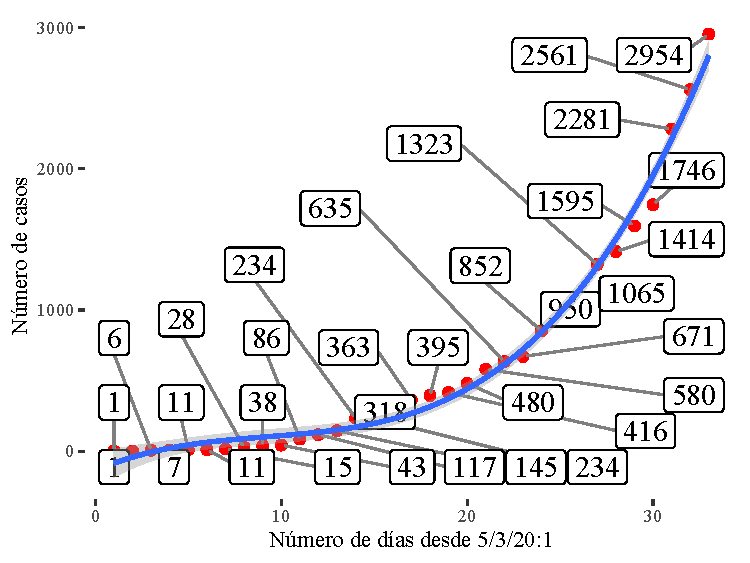
\includegraphics{E_1_files/figure-latex/ww1w-1} 

}

\caption{Regresión lineal}\label{fig:ww1w}
\end{figure}

\begin{verbatim}
## (Intercept) 
##    12917.13
\end{verbatim}

Sea la Tabla \ref{tab:2w3} Figures and tables with captions will be placed in \texttt{figure} and \texttt{table} environments, respectively.

\begin{longtable}[t]{cccccccccc}
\caption{\label{tab:2w3}Figures and tables with captions will be placed in `figure` }\\
\toprule
$Y_i$ & $f_i$ & $F_i$ & $F_i^*$ & $h_i$ & $H_i$ & $H_i^*$ & $h_i\%$ & $H_i\%$ & $H_i^*\%$\\
\midrule
ESTJ & 1 & 1 & 75 & 0.01 & 0.01 & 1.00 & 1.33 & 1.33 & 100.00\\
ESTJ & 2 & 3 & 150 & 0.03 & 0.04 & 2.00 & 2.67 & 4.00 & 200.00\\
ESTP & 3 & 6 & 150 & 0.04 & 0.08 & 2.00 & 4.00 & 8.00 & 200.00\\
ESFJ & 4 & 10 & 150 & 0.05 & 0.13 & 2.00 & 5.33 & 13.33 & 200.00\\
ESFP & 6 & 16 & 150 & 0.08 & 0.21 & 2.00 & 8.00 & 21.33 & 200.00\\
ISTJ & 6 & 22 & 155 & 0.08 & 0.29 & 2.07 & 8.00 & 29.33 & 206.67\\
ISTP & 7 & 29 & 157 & 0.09 & 0.39 & 2.09 & 9.33 & 38.67 & 209.33\\
ISFJ & 8 & 37 & 158 & 0.11 & 0.49 & 2.11 & 10.67 & 49.33 & 210.67\\
ISFP & 9 & 46 & 166 & 0.12 & 0.61 & 2.21 & 12.00 & 61.33 & 221.33\\
ENTJ & 10 & 56 & 166 & 0.13 & 0.75 & 2.21 & 13.33 & 74.67 & 221.33\\
ENTP & 6 & 62 & 166 & 0.08 & 0.83 & 2.21 & 8.00 & 82.67 & 221.33\\
ENFJ & 5 & 67 & 166 & 0.07 & 0.89 & 2.21 & 6.67 & 89.33 & 221.33\\
ENFP & 3 & 70 & 166 & 0.04 & 0.93 & 2.21 & 4.00 & 93.33 & 221.33\\
INTJ & 2 & 72 & 167 & 0.03 & 0.96 & 2.23 & 2.67 & 96.00 & 222.67\\
INTP & 1 & 73 & 169 & 0.01 & 0.97 & 2.25 & 1.33 & 97.33 & 225.33\\
INFJ & 1 & 74 & 172 & 0.01 & 0.99 & 2.29 & 1.33 & 98.67 & 229.33\\
INFP & 1 & 75 & 176 & 0.01 & 1.00 & 2.35 & 1.33 & 100.00 & 234.67\\
\bottomrule
\end{longtable}

  \bibliography{book.bib,packages.bib}

\printindex

\end{document}
